\chapter{Decodificación S/MIME desde Línea de Comandos}

\section{Descripción del proceso}

El estándar \textbf{S/MIME} (\textit{Secure/Multipurpose Internet Mail Extensions}) permite firmar y cifrar correos electrónicos mediante certificados X.509. Un mensaje que ha sido \textbf{cifrado y firmado} contiene una estructura anidada:

\begin{enumerate}
    \item \textbf{Capa externa -- Cifrado (SMIME.P7M):} El mensaje está cifrado con la clave pública del destinatario. Contiene un sobre PKCS\#7 (\texttt{application/pkcs7-mime; smime-type=enveloped-data}).
    \item \textbf{Capa interna -- Firma (SMIME.P7S):} Dentro del mensaje descifrado se encuentra la estructura firmada (\texttt{application/pkcs7-mime; smime-type=signed-data}), que contiene el texto original y la firma digital del emisor.
\end{enumerate}

Por tanto, el \textbf{descifrado} y la \textbf{verificación de la firma} han de realizarse \textbf{por separado} y en ese orden:

\begin{center}
    \texttt{.eml (P7M cifrado)} $\xrightarrow{\text{descifrar}}$ \texttt{.eml (P7S firmado)} $\xrightarrow{\text{verificar}}$ \texttt{texto plano}
\end{center}

\section{Ficheros necesarios}

Para el procesamiento se necesitan tres ficheros:

\begin{table}[H]
    \centering
    \caption{Ficheros necesarios para la decodificación S/MIME}
    \begin{tabularx}{\textwidth}{l|X}
        \toprule
        \textbf{Fichero} & \textbf{Descripción} \\
        \midrule
        Mensaje .eml & Correo cifrado y firmado, guardado como texto desde Thunderbird \\
        certificadoPersonal.crt + .key & Nuestro certificado y clave privada (para descifrar) \\
        WafaAzdadTriki.crt & Certificado de la compañera (para verificar su firma) \\
        \bottomrule
    \end{tabularx}
\end{table}

\section{Enunciado:}
1.3.1. Una vez el mensaje cifrado y firmado del compañero, se trata de decodificar ese mensaje desde la
utilidad ``openssl smime''. Para ello, hemos de guardar desde Thunderbird el mensaje completo como texto en
formato ``.eml'' (seleccionar mensaje, botón de la derecha, Guardar cómo\dots), exportar nuestro certificado
completo (o utilizar nuestro fichero \texttt{certificadoPersonal.p12}) y el certificado del compañero (Exportar en
formato \texttt{.crt}) y procesar estos tres ficheros (mensaje de texto y los dos certificados) a través de la citada
utilidad ``openssl smime''.

1.3.2. El apartado 5.- S/MIME de la Wiki explica con detalle cómo procesar correos S/MIME desde línea de
comandos openssl, lo que pedimos ahora está explicado en el apartado 5.2.4. -- Descifrar mensaje cifrado y
firmado de la citada Wiki. Obsérvese que el descifrado y la verificación de firma han de hacerse por
separado. Documentar este proceso en detalle, mostrando en capturas de pantalla la cabecera de correo
con los adjuntos, tanto del fichero cifrado y firmado (SMIME.P7M) como del fichero resultado de
descifrado (SMIME. P7S).

\section{Paso 1 -- Descifrado del mensaje (SMIME.P7M $\rightarrow$ SMIME.P7S)}

Se utiliza \texttt{openssl smime -decrypt} con nuestro certificado personal y clave privada, ya que el mensaje fue cifrado con nuestra clave pública:

\begin{lstlisting}[caption=Descifrado del mensaje S/MIME]
openssl smime -decrypt \
    -in "mensaje_wafa.eml" \
    -recip certificadoPersonal.crt \
    -inkey certificadoPersonal.key \
    -out mensaje_descifrado.eml
\end{lstlisting}

\textbf{Parámetros:}
\begin{itemize}[label=\textbullet]
    \item \texttt{-in}: Fichero .eml con el mensaje cifrado (contiene el SMIME.P7M).
    \item \texttt{-recip}: Nuestro certificado personal en formato PEM (.crt), que corresponde a la clave pública con la que se cifró el mensaje.
    \item \texttt{-inkey}: Nuestra clave privada (.key), protegida con contraseña.
    \item \texttt{-out}: Fichero de salida con el contenido descifrado (contiene el SMIME.P7S, es decir, la estructura firmada).
\end{itemize}

\textbf{Nota:} El parámetro \texttt{-recip} requiere el certificado en formato PEM (\texttt{.crt}) en macOS, {no} el fichero PKCS\#12 (\texttt{.p12}). Si solo se dispone del \texttt{.p12}, hay que extraer primero el certificado y la clave.
Sin embargo, al realizar la captura en Kali Linux, se pudo usar el fichero \texttt{.p12} directamente con \texttt{-recip}, lo que sugiere una diferencia en la implementación de OpenSSL entre ambos sistemas operativos.

El resultado es un fichero \texttt{.eml} que contiene la cabecera MIME del mensaje firmado, con el adjunto \texttt{smime.p7s} visible.

\section{Paso 2 -- Verificación de la firma (SMIME.P7S $\rightarrow$ texto plano)}

Se utiliza \texttt{openssl smime -verify} con el certificado de la compañera para comprobar que el mensaje fue firmado por ella y no ha sido alterado:

\begin{lstlisting}[caption=Verificación de la firma S/MIME]
openssl smime -verify \
    -in mensaje_descifrado.eml \
    -signer WafaAzdadTriki.crt \
    -CAfile certificadoRaiz.crt \
    -out mensaje_plano.txt
\end{lstlisting}

\textbf{Parámetros:}
\begin{itemize}[label=\textbullet]
    \item \texttt{-in}: Fichero descifrado que contiene la estructura firmada (SMIME.P7S).
    \item \texttt{-signer}: Certificado del firmante (la compañera) para verificar la firma.
    \item \texttt{-CAfile}: Certificado de la CA raíz. Si ambos usamos la misma CA raíz de la asignatura, la verificación completa funciona. Si la CA es externa o no se dispone de ella, se usa \texttt{-noverify} en su lugar.
    \item \texttt{-out}: Fichero de salida con el texto plano del mensaje.
\end{itemize}

Si el certificado de la compañera fue emitido por una CA diferente, la verificación de cadena fallará con el error \texttt{unable to get local issuer certificate}. En ese caso se puede usar el flag \texttt{-noverify} para omitir la verificación de la cadena de CA y comprobar únicamente la firma:

\begin{lstlisting}[caption=Verificación sin comprobación de cadena de CA]
openssl smime -verify \
    -in mensaje_descifrado.eml \
    -signer WafaAzdadTriki.crt \
    -noverify \
    -out mensaje_plano.txt
\end{lstlisting}

\section{Resultado del proceso}

\begin{figure}[H]
    \centering
    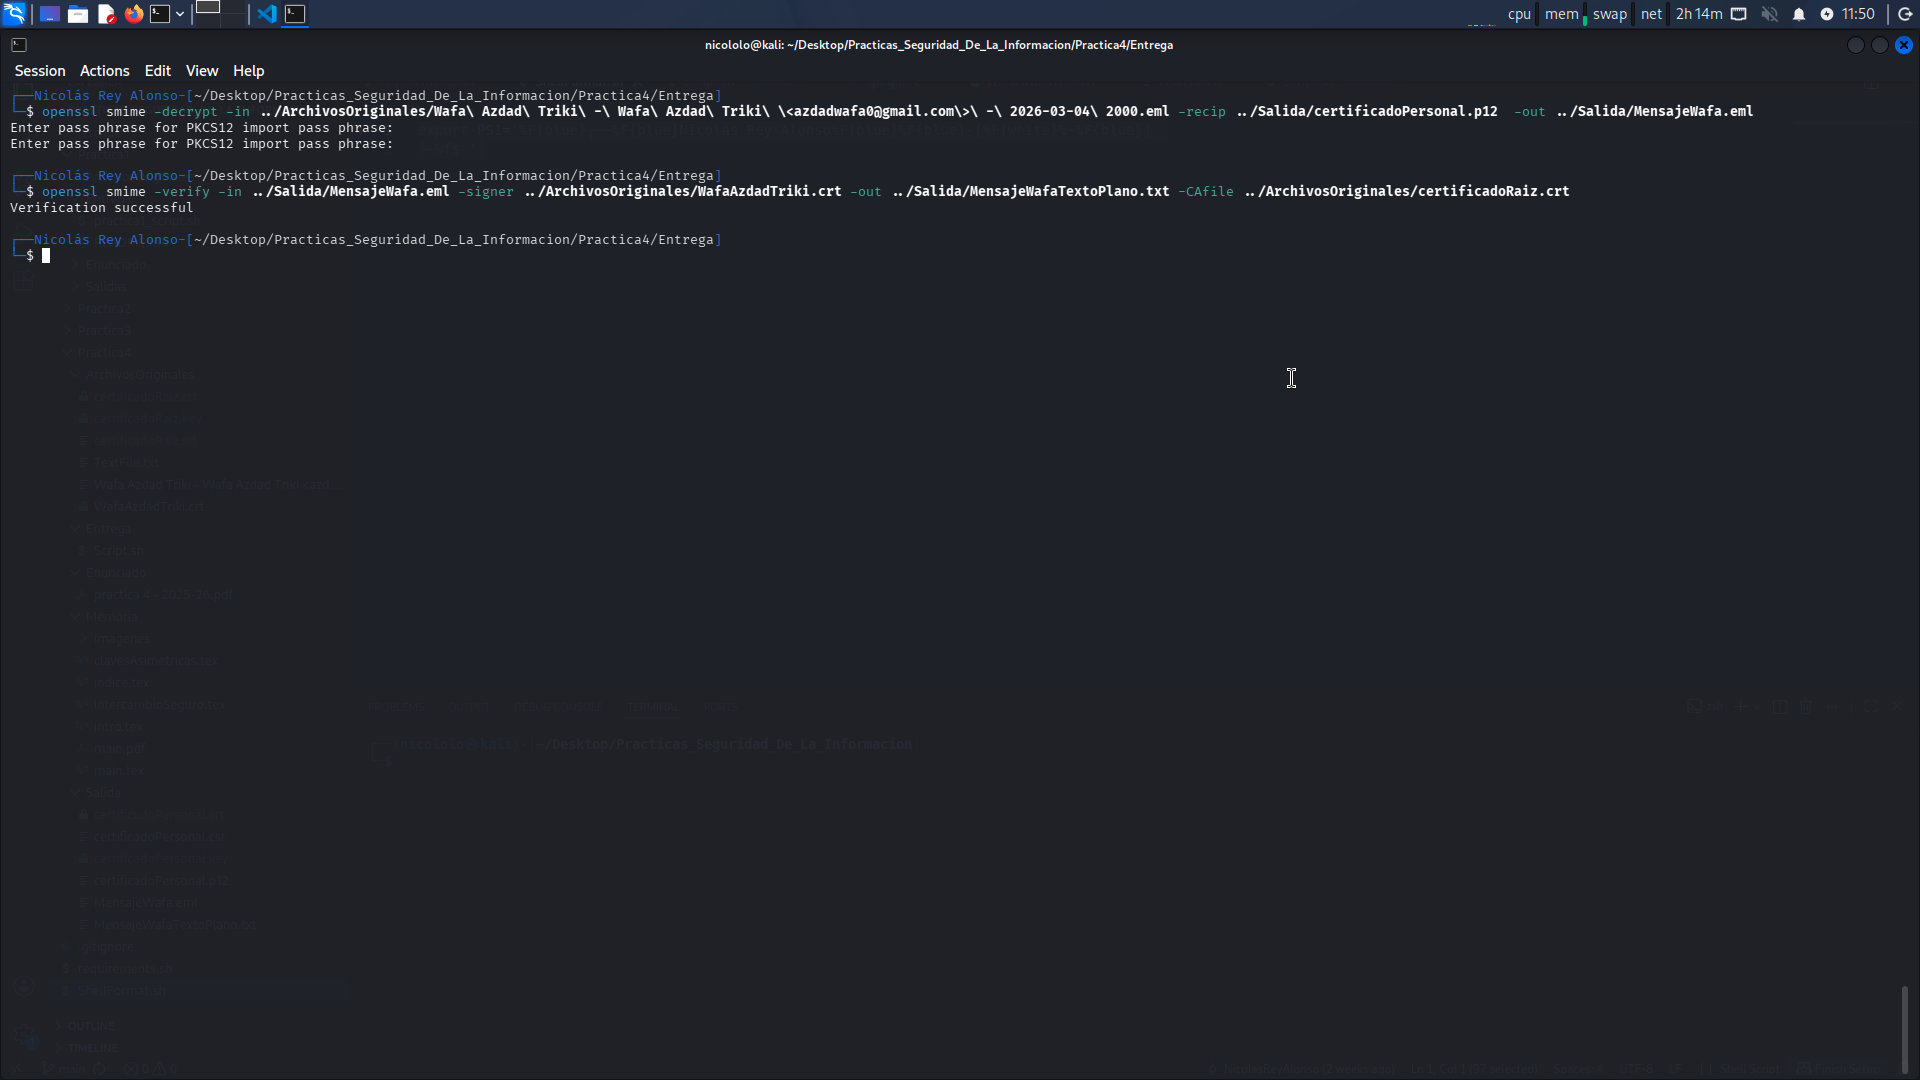
\includegraphics[width=\textwidth]{Imagenes/Descifrar_Y_Verificar_Wafa_Terminal.png}
    \caption{Proceso completo de descifrado y verificación de firma en terminal}
    \label{fig:descifrar_verificar}
\end{figure}

La verificación exitosa muestra el mensaje \texttt{Verification successful}, confirmando que:

\begin{itemize}[label=\textbullet]
    \item El mensaje fue efectivamente firmado por la compañera (autenticación del origen).
    \item El contenido no ha sido alterado desde su firma (integridad).
\end{itemize}

El contenido del mensaje descifrado y verificado se muestra a continuación:

\begin{figure}[H]
    \centering
    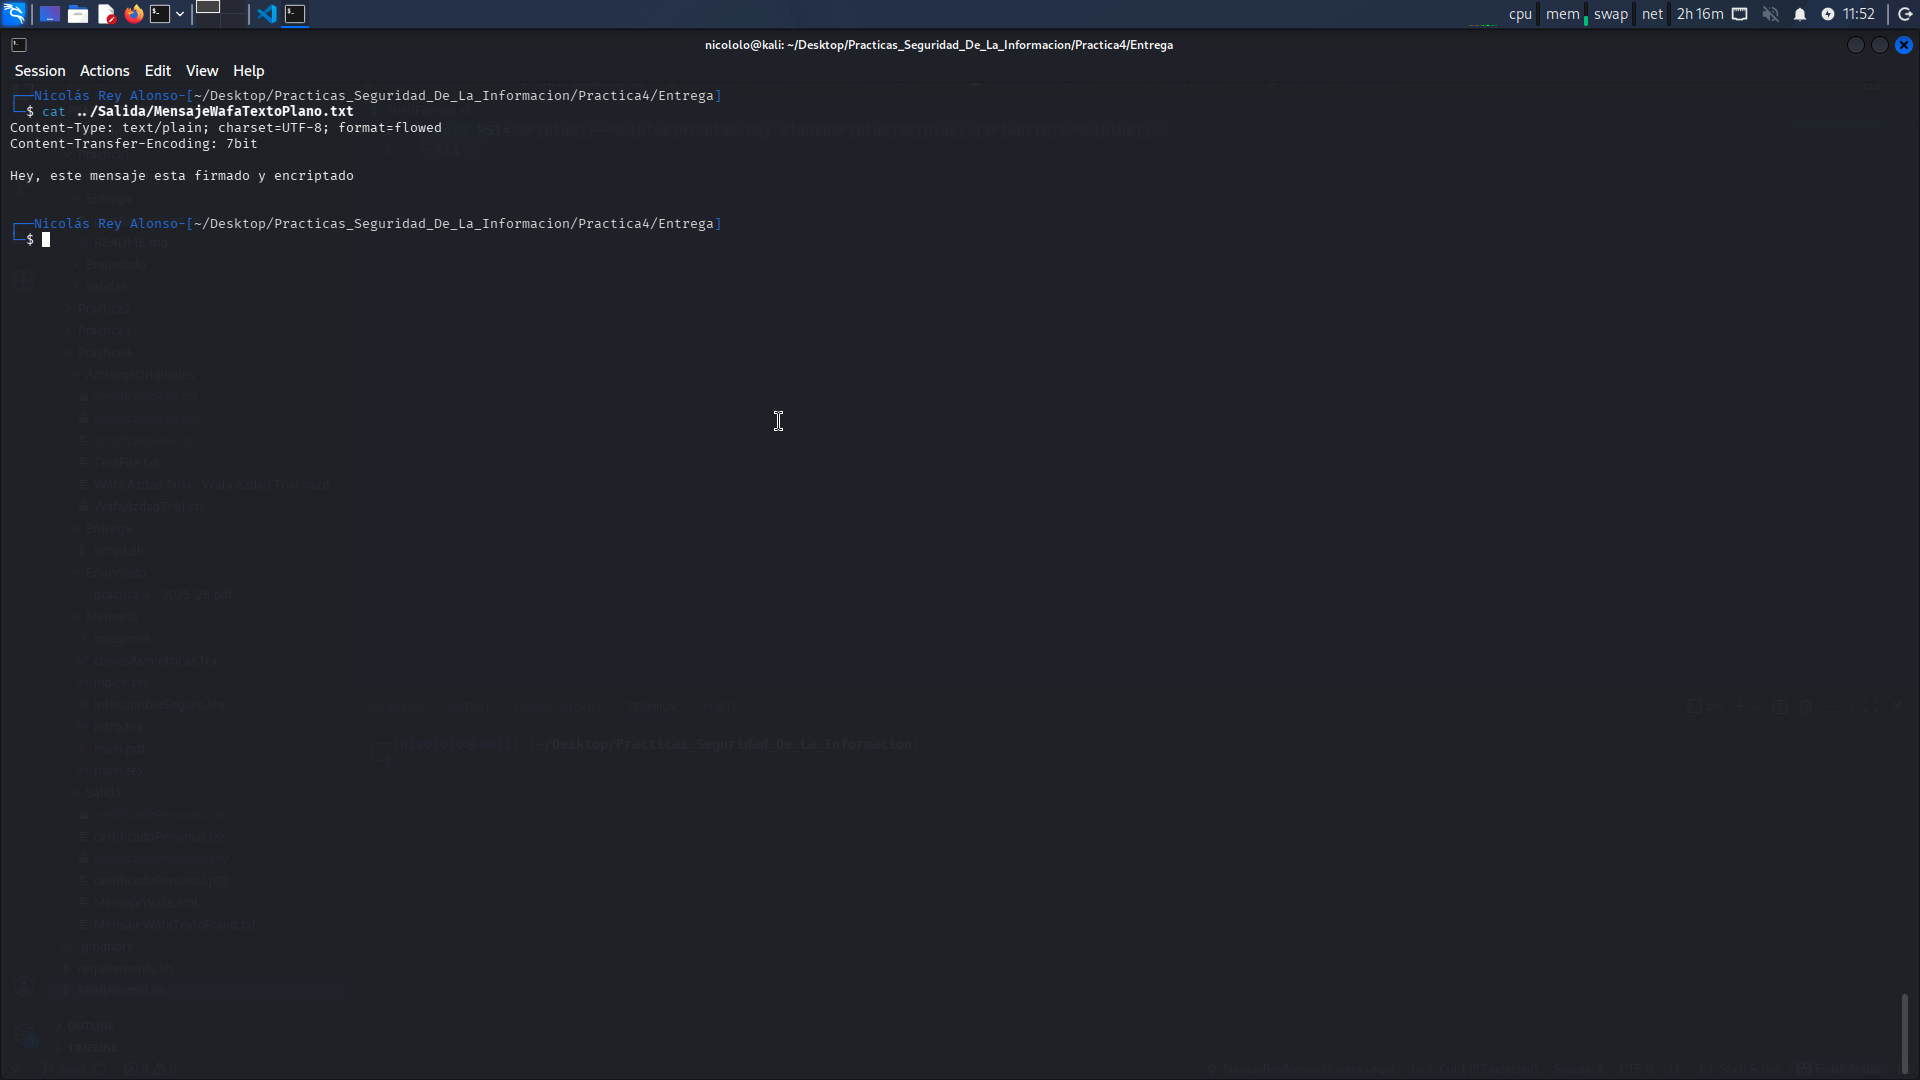
\includegraphics[width=\textwidth]{Imagenes/ContenidoDescifradoEnTerminal.png}
    \caption{Contenido del mensaje descifrado y verificado en texto plano}
    \label{fig:contenido_descifrado}
\end{figure}

\section{Resumen del flujo completo}

\begin{table}[H]
    \centering
    \caption{Resumen de operaciones S/MIME}
    \begin{tabularx}{\textwidth}{c|l|l|X}
        \toprule
        \textbf{Paso} & \textbf{Operación} & \textbf{Comando} & \textbf{Claves utilizadas} \\
        \midrule
        1 & Descifrar & \texttt{smime -decrypt} & Certificado y clave privada propios \\
        2 & Verificar firma & \texttt{smime -verify} & Certificado del firmante (compañera) \\
        \bottomrule
    \end{tabularx}
\end{table}

Este proceso demuestra el \textbf{esquema de doble envolvente} de S/MIME: primero se firma el mensaje (garantizando autenticación e integridad), y luego se cifra el resultado (garantizando confidencialidad). Al recibirlo, se deshacen las capas en orden inverso: primero descifrado, luego verificación de firma.
